\section*{Appendix: Evolution of Distinction in Small-World Transitions}
\label{sec:appendix-small-world}

To further understand the structural behavior of the distinction centrality measure, we conduct a computational experiment simulating the transition from a perfectly symmetric, highly constrained structure to a fully saturated, completely connected structure. We trace how structural inequality (variance in scaled distinction) and structural dependence (mean constraint) evolve.

\subsection*{Simulation Setup}

We begin with a regular lattice graph (a circle graph or ring) of size $N = 30$. Because the graph is node-transitive, every node is structurally equivalent, yielding an identical initial eigenvector status. Under the absolute maximum (\texttt{abm}) normalization, deleting any node results in the identical residual $N-1$ path graph. Thus, at this initial state, all nodes experience identical constraint, and the variance in scaled distinction is exactly zero.

From this initial state, we progressively add non-existent edges at random until the graph becomes a complete graph ($K_{30}$). Figure \ref{fig:small-world-snapshots} visualizes three structural snapshots from this process: the initial symmetric lattice, a sparse small-world phase characterized by a few random shortcuts, and a much denser random graph approaching full connectivity. At each step of the simulation, we recalculate the distinction metrics for the network and record both the standard deviation of the scaled distinction ($\beta_i$) and the mean of the constraint ($\kappa_i$) across all nodes as a function of the network's density.

\begin{figure}[ht!]
    \centering
    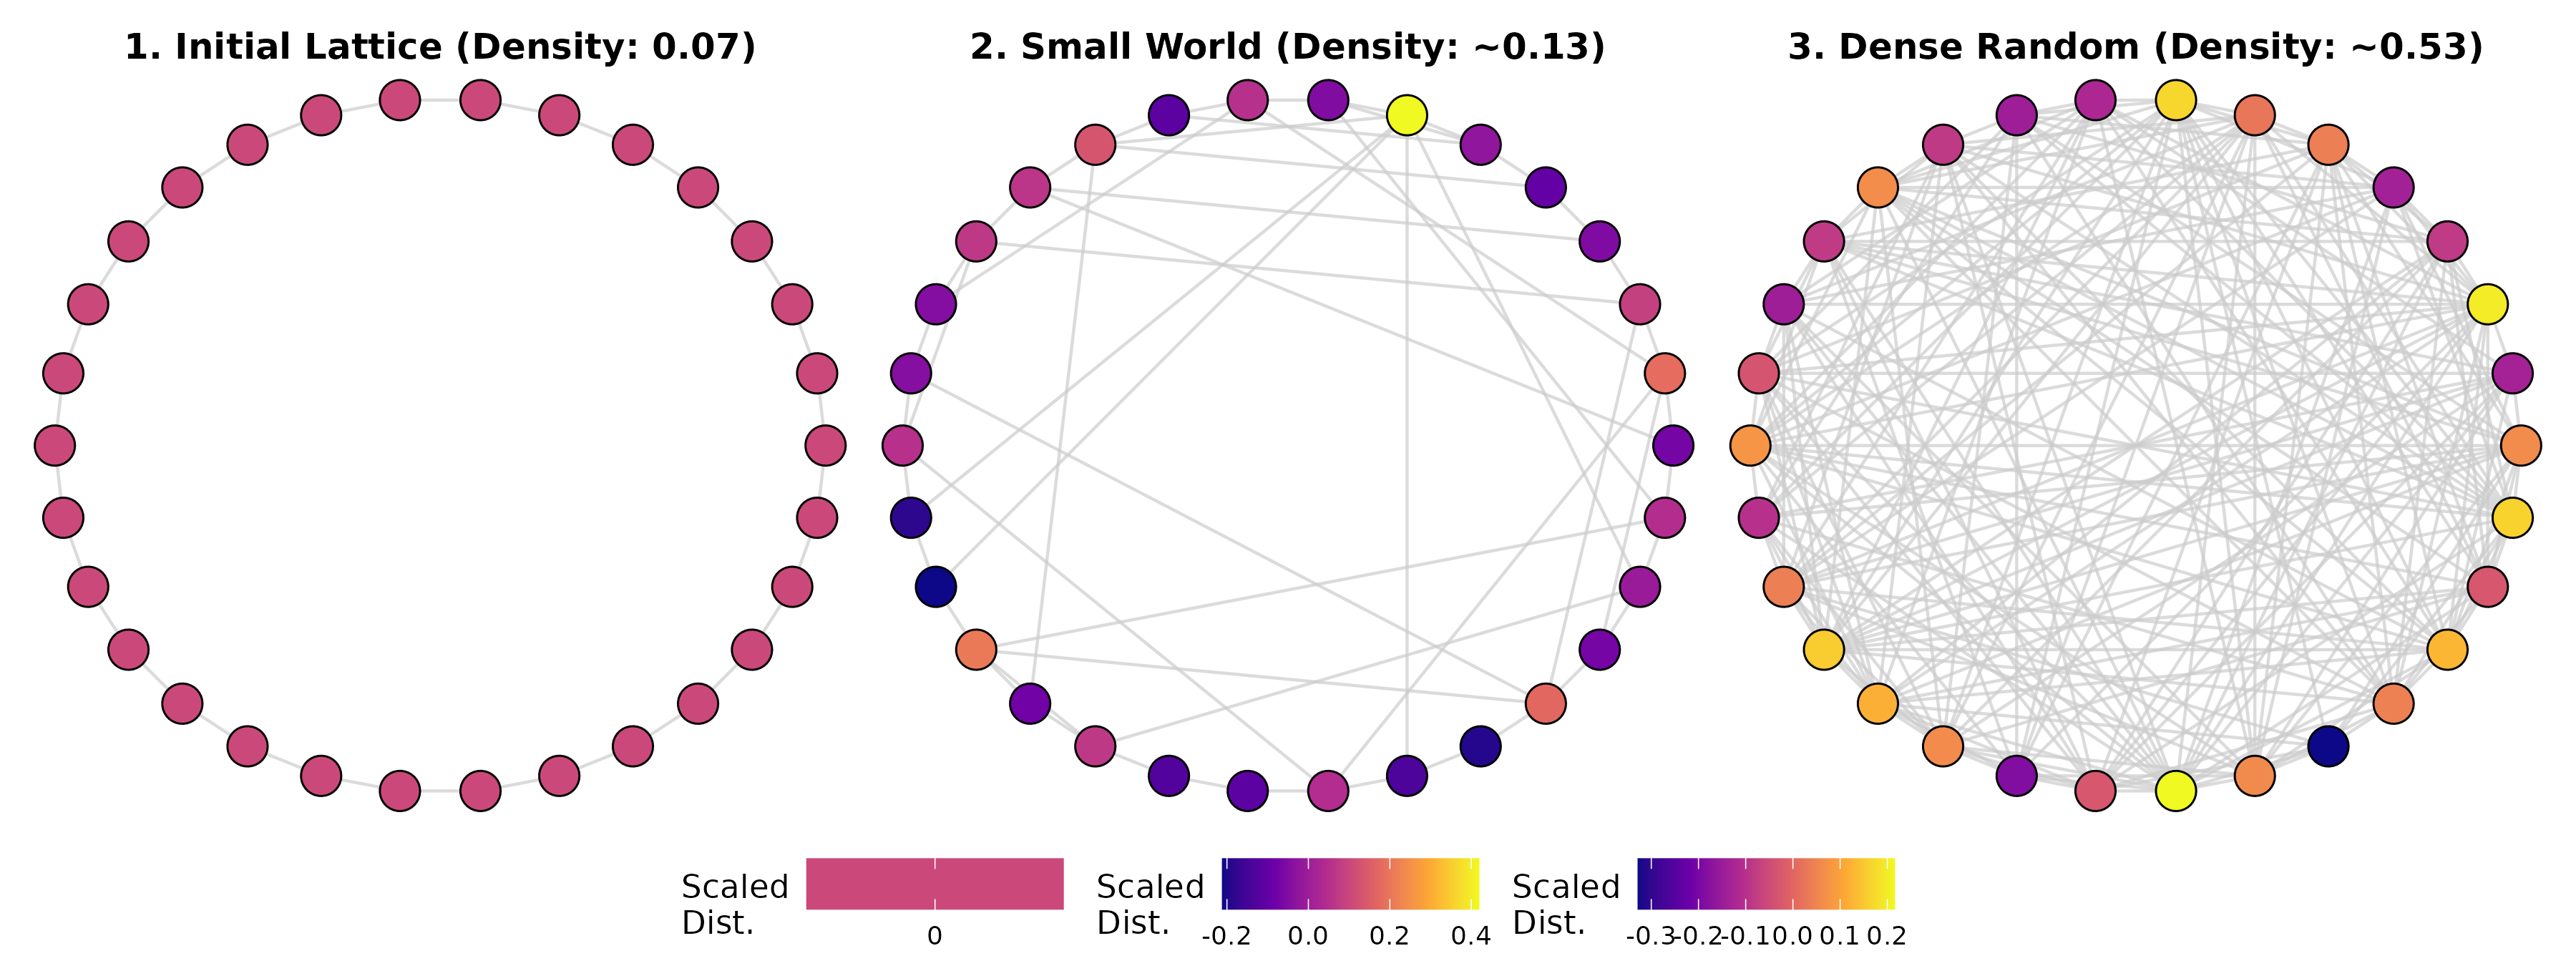
\includegraphics[width=\linewidth]{Plots/small_world_snapshots.png}
    \caption{Three snapshots from the small-world computational experiment ($N=30$), varying from the initial symmetric lattice to a dense random graph. Nodes are colored by their scaled distinction score.}
    \label{fig:small-world-snapshots}
\end{figure}

\subsection*{Results}

Figure \ref{fig:variance-density} shows the variance of the scaled distinction scores as network density increases. The variance follows a clear inverted U-shape.
At zero density (the regular lattice) and full density (the complete graph), the variance is zero. Both configurations represent extreme forms of structural equality—the former through maximum local constraint, the latter through maximum structural saturation and redundancy. 

\begin{figure}[ht!]
    \centering
    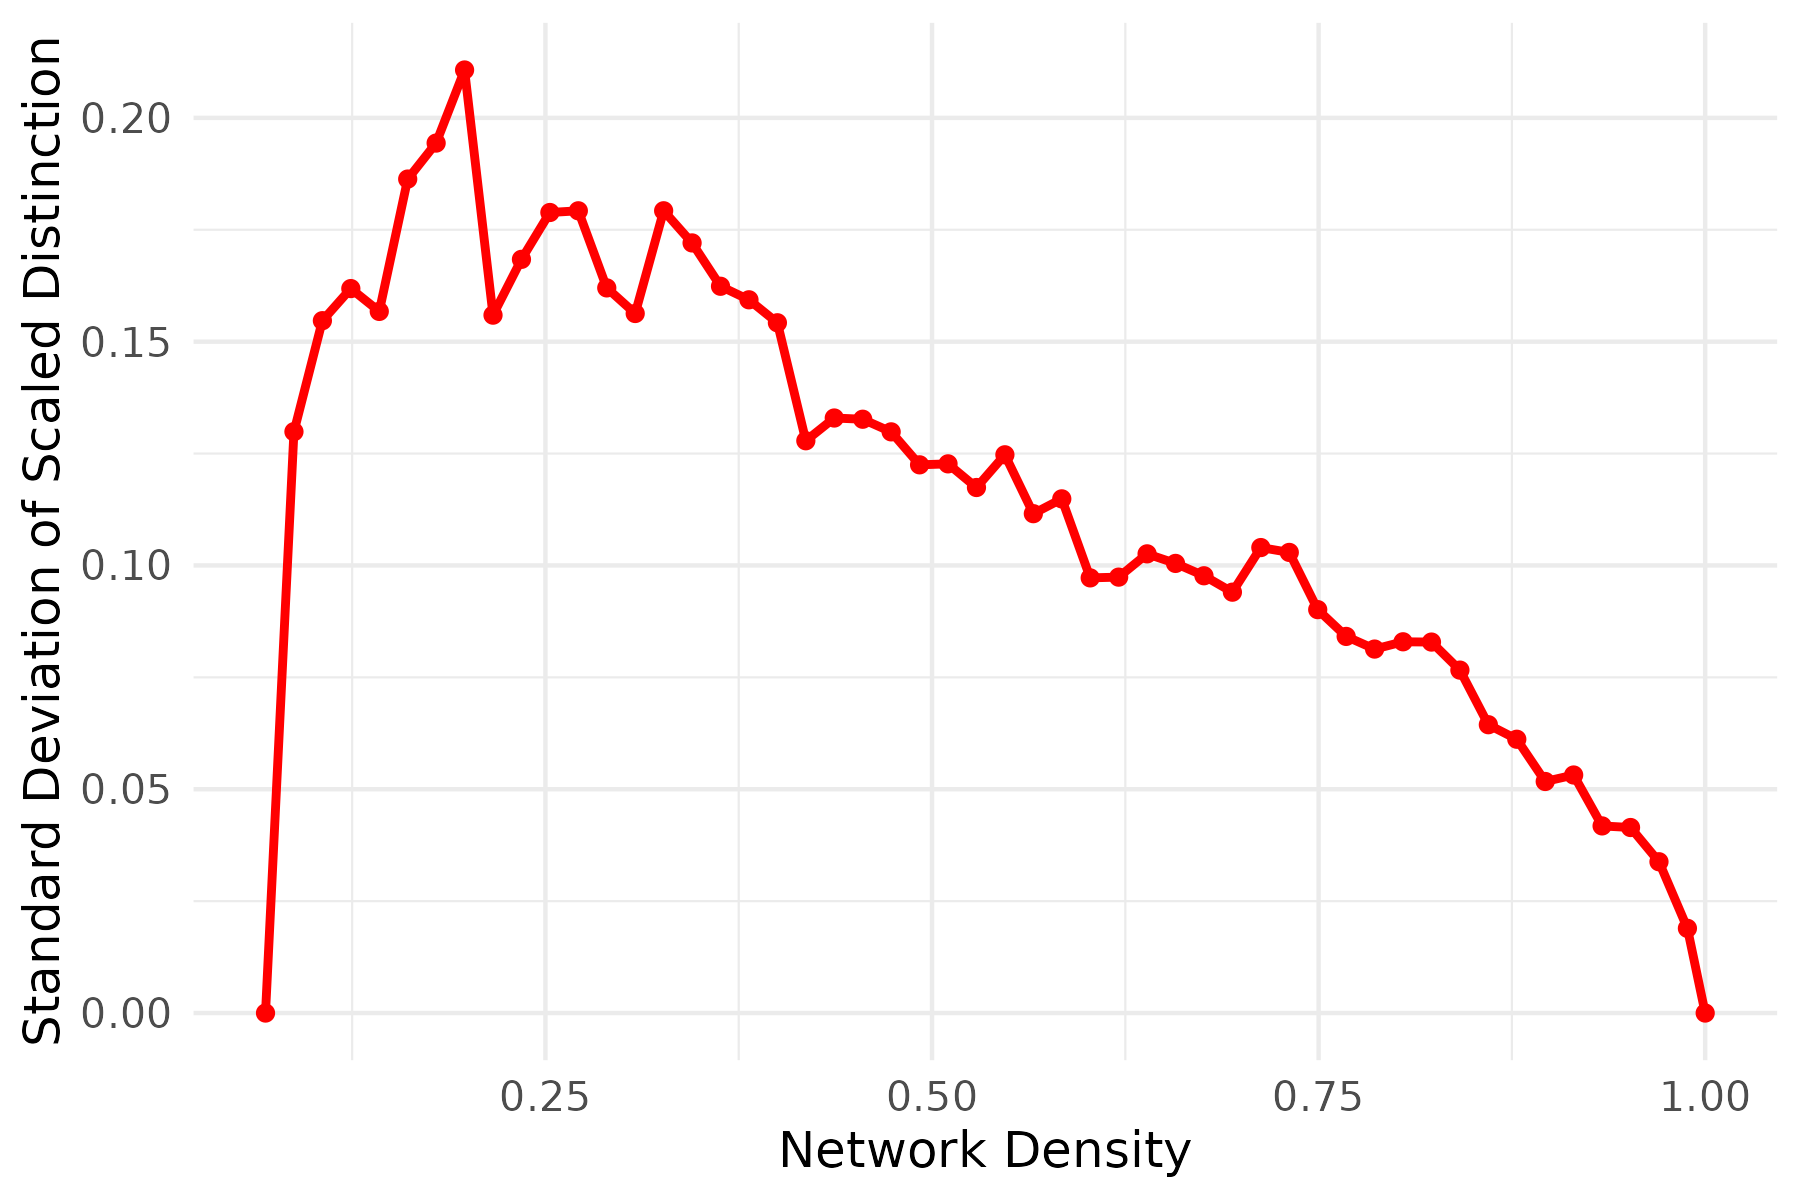
\includegraphics[width=0.6\linewidth]{Plots/variance_vs_density.png}
    \caption{Variance (standard deviation) of scaled distinction as edges are randomly added to a regular lattice.}
    \label{fig:variance-density}
\end{figure}

However, as the first random long-ties are added to the lattice—mimicking the emergence of a small-world topology—structural inequality skyrockets. A few nodes become highly distinctive brokers while others remain locally constrained within the lattice. The variance of distinction hits its absolute maximum in this sparse, clumpy regime (around a density of 0.15 to 0.25). As more edges are continuously added, the structural advantages of the early brokers are diluted by the emergence of redundant pathways, and the variance of distinction steadily declines back to zero.

Figure \ref{fig:mean-constraint-density} plots the evolution of the mean baseline constraint. Mean constraint follows a monotonically increasing curve. It starts at its lowest point in the regular lattice. As edges are added, the mean constraint rises steadily because nodes are increasingly connected to alters with heterogeneous and higher status scores, thereby increasing the structural dependence on neighbors. This constraint eventually asymptotes to exactly $1.0$ in the complete graph, where the deletion of any node leaves a complete graph of $N-1$, ensuring all remaining neighbors have maximum status.

\begin{figure}[ht!]
    \centering
    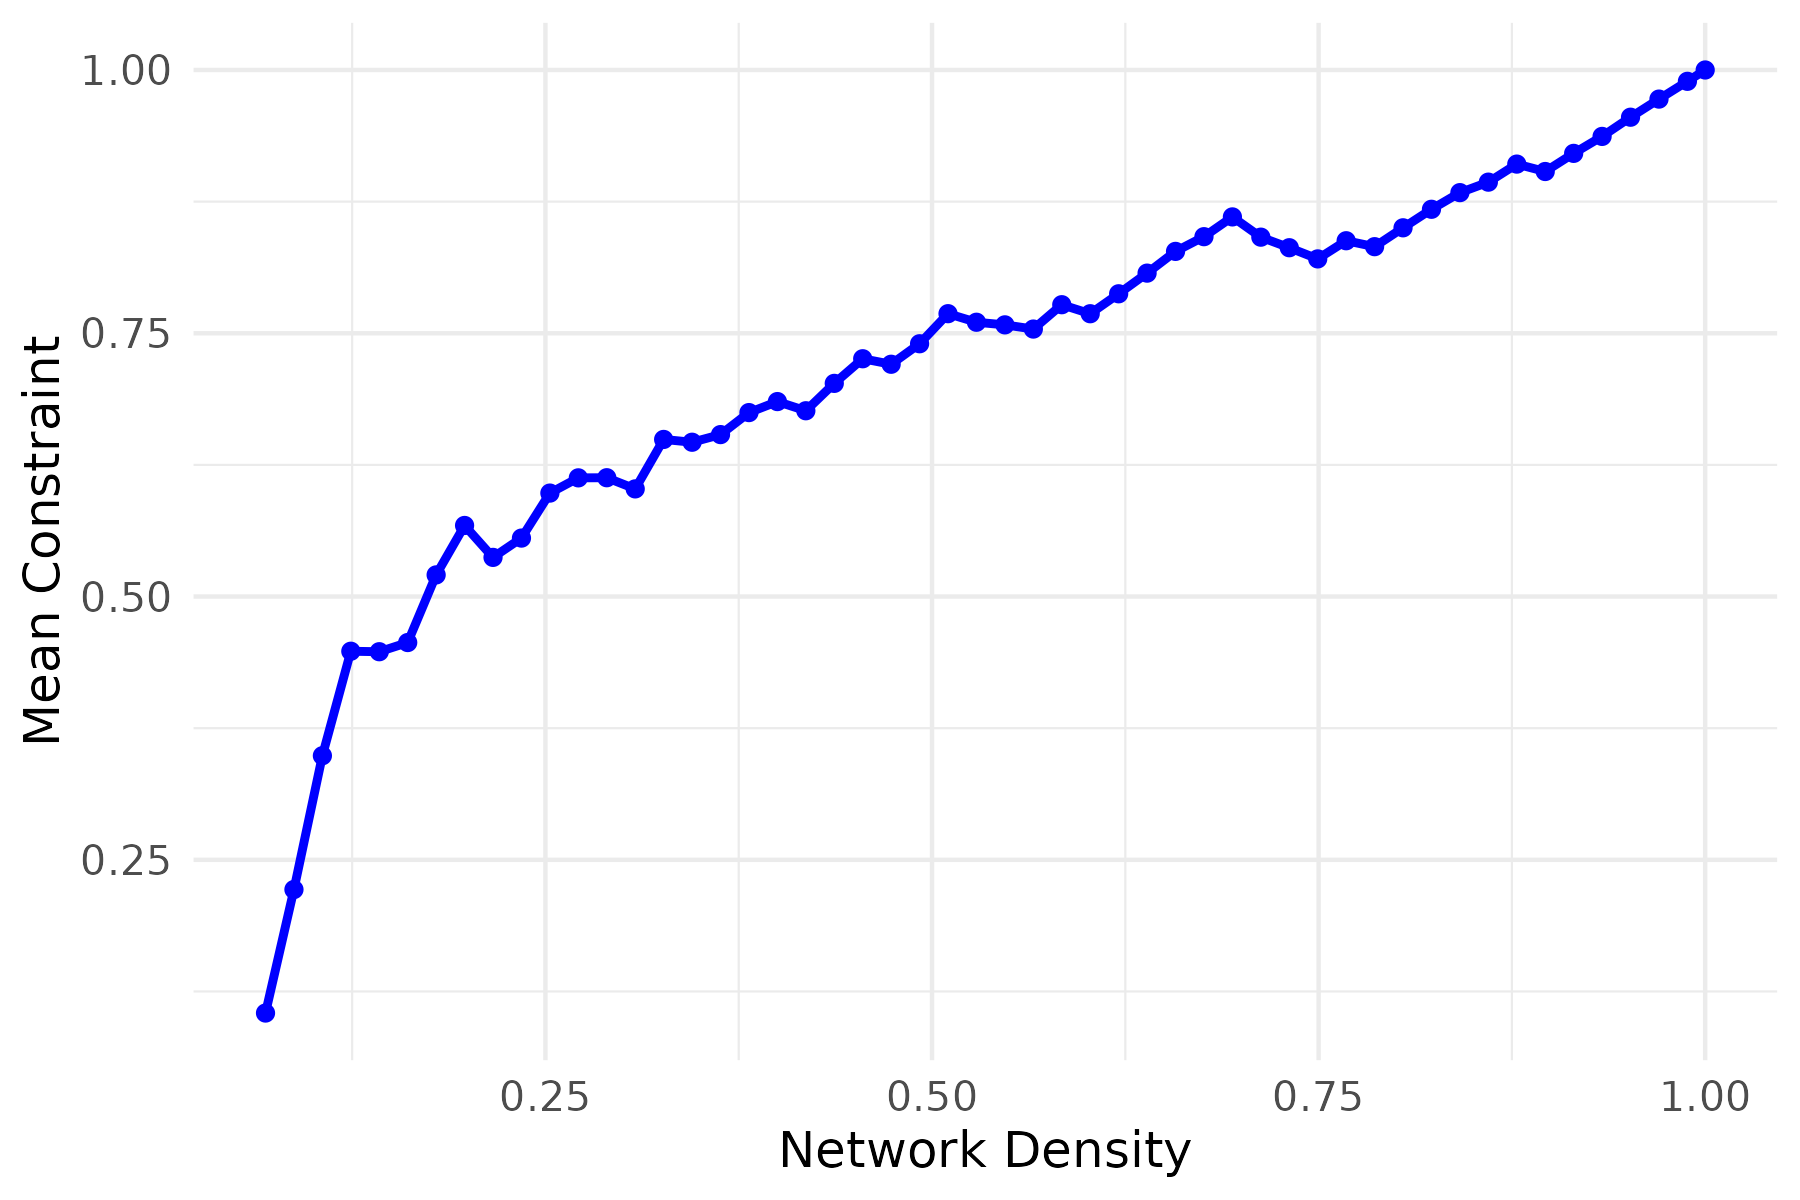
\includegraphics[width=0.6\linewidth]{Plots/mean_constraint_vs_density.png}
    \caption{Evolution of mean constraint ($\kappa$) as edges are randomly added to a regular lattice.}
    \label{fig:mean-constraint-density}
\end{figure}

These evolutionary dynamics perfectly mirror theoretical expectations of agonistic fields: perfect structural equality exists only at the extremes of total constraint or total saturation. Inequality in distinction peaks precisely in the intermediate, sparse ``small-world'' phase where a subset of actors successfully monopolize structural bridging.
